\section{Data Acquisition}

Data acquisition from both the FSR sensors and the Shimmer3 devices are set to have a sample frequency of 100Hz. This sample rate is used by others performing similar measurements \cite{Verkerke2005, Byun2016, Sherwani2016}. Additionally, the sample rate is decided to be the same so it is possible to match the two data streams to each other, so it is possible to compare measured pressure forces under the feet while matching it to movement of the body. A simple graphical user interface (GUI) have been developed to match the data. This manual approach is favourable for this project as it were determined that it would be more time consuming to develop an algorithm to automatically match data streams. It would also go beyond the scope for the project.

Data from the Shimmer3 devices are send and saved directly to MATLAB via Bluetooth and stored in $n\times3$ matrices, one for each leg.

For saving acquired data from the FSR sensors an Arduino program have been written to arrange measurements into an $n\times6$ matrix. Each column corresponds with the channel input for each FSR. See \figref{fig:FSRNumbering} for the numbering of FSRs and channels. Rows in the matrix are time steps. The data is saved to a $.txt$-file on the microSD card. 

\begin{figure}[H]
	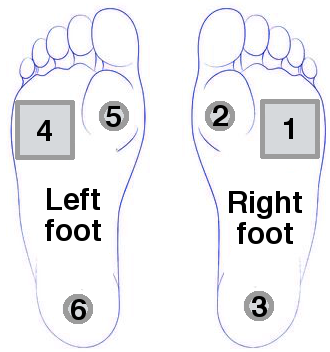
\includegraphics[width=.6\textwidth]{figures/FSRNumbering}
	\caption{The numbering of each FSR sensor according to the channel they are recorded to in the Arduino program.}
	\label{fig:FSRNumbering}  %<--remember LABEL!
\end{figure}



